%
% wavelet.tex
%
% (c) 2019 Prof Dr Andreas Müller, Hochschule Rapperswil
%
\section{Wavelet%
\label{section:haar-wavelet}}
\rhead{Wavelet}
Im vorangegangenen Abschnitt wurde die Menge $\mathbb D$ konstruiert, die
einerseits ``grobe'' Unterteilungen $U_j$ für kleines $j$ enthält, die ohne
grossen Abtastaufwand eine grobe Darstellung des Signals ermöglicht,
andererseits für grosses $j$ aber auch beliebig ``feine'' Unterteilungen
enthält, mit denen das Signal beliebig genau wiedergegeben werden kann.
Die bereits erfassten ``groben'' Abtastwerte passen zudem genau in die
``feinen'' Abtastreihen.

\begin{figure}
\centering
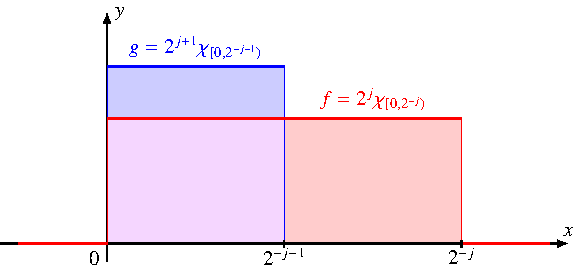
\includegraphics{chapters/3-haar/images/ortho.pdf}
\caption{Die Funktion $f$ und $g$ von \eqref{haar:formel:ortho} sind
nicht orthogonal.
Dies zeigt, dass die Indikatorfunktionen von Zweierpotenzintervallen
keine orthonormierte Basis sein können.
\label{haar:figure:ortho}}
\end{figure}
Wir haben auch versucht, eine orthonormierte Basis für die Vektorräume
$V_j$ der Signale zu konstruieren.
Natürlich bilden die einzelnen in $V_j$ gefundenen Basisfunktionen eine 
Hilbert-Basis des Vektorraumes $V_\infty$, aber die Funktionen sind
nicht orthogonal.
Zum Beispiel haben die Funktionen 
\begin{equation}
\begin{aligned}
f&=2^{j/2}\chi_{[0,2^{-j})}
\\
g&=2^{(j+1)/2}\chi_{[0,2^{-j-1})},
\end{aligned}
\label{haar:formel:ortho}
\end{equation}
(Abbildung~\ref{haar:figure:ortho})
das nicht verschwindende Skalarprodukt
\[
\langle f,g\rangle 
=
\int_{-\infty}^\infty
2^{j/2}\chi_{[0,2^{-j})}(x)
2^{(j+1)/2}\chi_{[0,2^{-j-1})}(x)\,dx
=
\int_0^{2^{-j-1}} 2^{j/2}\cdot 2^{(j+1)/2}\,dx
=
2^{-j-1}2^{j + 1/2}
=
\frac{1}{\sqrt{2}}\ne 0.
\]
Das Sampling mit der Funktion $g$ nimmt einen Teil der Information,
die das Sampling mit $f$ schon ermittelt hat, nochmals auf.

\subsection{Detail auf Ebene $j$}
\begin{figure}
\centering
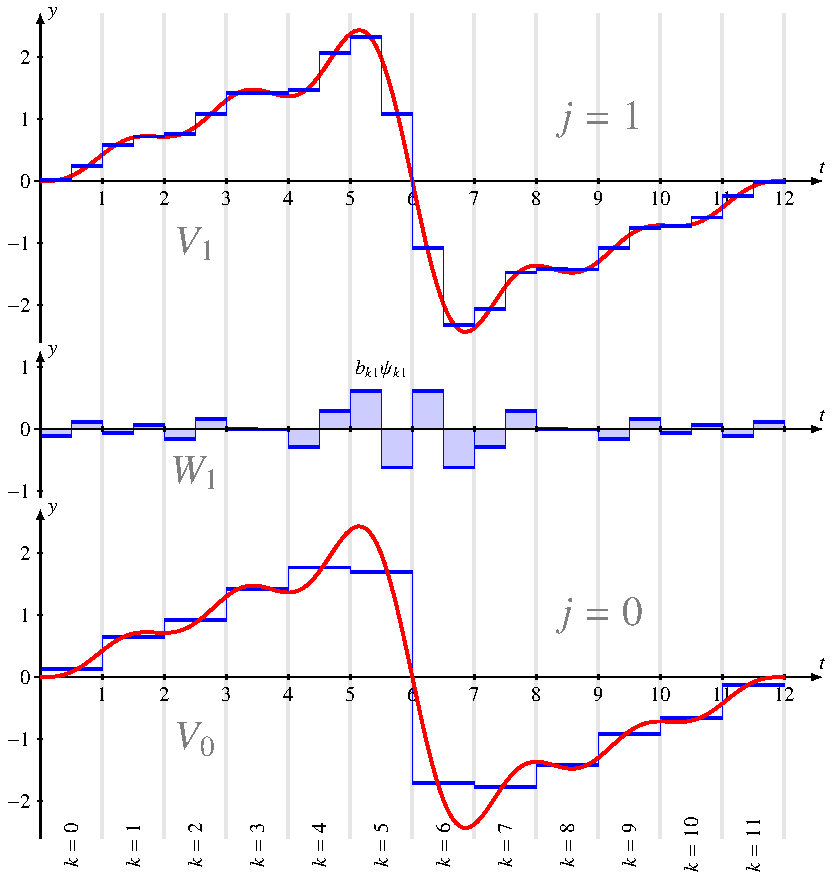
\includegraphics{chapters/3-haar/images/detail.pdf}
\caption{Analyse der Funktion $\color{red}f(t)$ mit dem Haar-Wavelet.
Die Analyse in $V_0$ ergibt eine auf Intervallen der Länge 1 stückweise
konstante Funktion mit Funktionswerten, die den Mittelwerten der Funktion
über diese Intervalle entsprechen.
In $V_1$ erhält man eine auf Intervallen der Länge $\frac12$ stückweise
konstante Funktion.
Der Unterschied ist eine Funktion, die aus $\psi_{1k}\in W_1$ linear
kombiniert wurde.
Die Koeffizienten $b_{k1}$ geben die zusätzlichen Details wieder,
die in der Auflösung $2^{-1}$ sichtbar werden.
\label{haar:figure:detail}}
\end{figure}
Um eine orthonormierte Basis von $V_\infty$ zu erhalten, müssen
bei der Erweiterung von $V_j$ zu $V_{j+1}$ neue, auf den bisherigen
orthogonale Basisfunktionen konstruiert werden, die nur die neue
Information aufnehmen, die die feinere Unterteilung in $V_{j+1}$
zu erfassen in der Lage ist.

In Abbildung~\ref{haar:figure:detail} ist eine Funktion dargestellt mit
der Approximation in $V_0$ unten und $V_1$ oben.
Der Unterschied zwischen den Approximation ist die zusätzliche
Detailinformation auf Ebene $j+1$.
Das Ziel ist, diesen Unterschied als Linearkombination von orthonormierten
Funktionen $\psi_{jk}$ zu beschreiben.

Das Sampling eines Signals $f(x)$ mit der Funktion $e^{(l)}$ in $V_j$
ermittelt das Integral
\[
\langle f,e^{(l)}\rangle
=
2^{j/2}
\int_{l2^{-j}}^{(l+1)2^{-j}} f(x)\,dx,
\]
also im wesentlichen den Mittelwert über das Intervall $[l2^{-j},(l+1)2^{-j})$.
Veränderungen des Signals innerhalb des Intervalls sind in $V_j$ nicht
auflösbar.
Beim Sampling in $V_{j+1}$ stehen zwei Basisfunktionen zur Verfügung, die
den gleichen Bereich abdecken.
Jede dieser Basisfunktionen ermittelt das Integral über eine Hälfte des
Intervalls.
Veränderungen innerhalb der Intervallhälften sind in $V_{j+1}$ wieder nicht
erkennbar.
Die neue Information in $V_{j+1}$ ist, wie sich der Mittelwert
in der ersten Intervallhälfte vom Mittelwert in der zweiten Intervallhälfte
unterscheidet, also die Differenz
\[
\int_{l2^{-j}}^{(l+\frac12)2^{-j}} f(x)\,dx
-
\int_{(l+\frac12)2^{-j}}^{(l+1)2^{-j}} f(x)\,dx.
\]
Dies lässt sich als ein Skalarprodukt
\[
\langle f,
\chi_{[l2^{-j},(l+\frac12)2^{-j})}
-
\chi_{[(l+\frac12)2^{-j},(l+1)2^{-j})}
\rangle
\]
schreiben.
Die Funktion rechts im Skalarprodukt ist also diejenige, die genau die
neue Information in $V_{j+1}$ ermittelt.

Die eben angestellte heuristische Überlegung legt nahe, dass die Funktionen
\begin{equation}
\chi_{[l2^{-j},(l+\frac12)2^{-j})}
-
\chi_{[(l+\frac12)2^{-j},(l+1)2^{-j})}
\end{equation}
zu den Basisfunktionen, die man in $V_j$ bereits hat, hinzugefügt werden
müssen.
Allerdings sind diese Funktionen noch nicht orthonormiert, denn die
Norm ist
\[
\|
\chi_{[l2^{-j},(l+\frac12)2^{-j})}
-
\chi_{[(l+\frac12)2^{-j},(l+1)2^{-j})}
\|^2
=
\int_{-\infty}^\infty
|
\chi_{[l2^{-j},(l+\frac12)2^{-j})}
-
\chi_{[(l+\frac12)2^{-j},(l+1)2^{-j})}
|^2
\,dx
=
2^{-j}.
\]
Wir verwenden daher die Funktionen
\[
\psi_{jl}(x) = 2^{j/2}(
\chi_{[l2^{-j},(l+\frac12)2^{-j})(x)}
-
\chi_{[(l+\frac12)2^{-j},(l+1)2^{-j})(x)}
)
\]
als Basis.
Um dies zu rechtfertigen, muss gezeigt werden, dass diese Funktionen auf
allen Funktionen in $V_j$ orthogonal und auch untereinander orthogonal
sind.

\subsection{Orthogonalität}
Betrachten wir erst die Frage, ob die Funktionen untereinander orthonormiert
sind.
$\psi_{jl}(x)$ ist nur im Intervall $[l2^{-j},(l+1)2^{-j})$ von $0$
verschieden.
Zwei Funktionen $\psi_{jl}(x)$ und $\psi_{jk}(x)$ mit $l\ne k$ sind
also nirgends gleichzeitig von $0$ verschieden, das Skalarprodukt ist
daher $0$.
Dass das Skalarprodukt von $\psi_{jl}(x)$ mit sich selbst $1$ ist wurde
durch die oben gewählte Normierung sichergestellt.

\begin{figure}
\centering
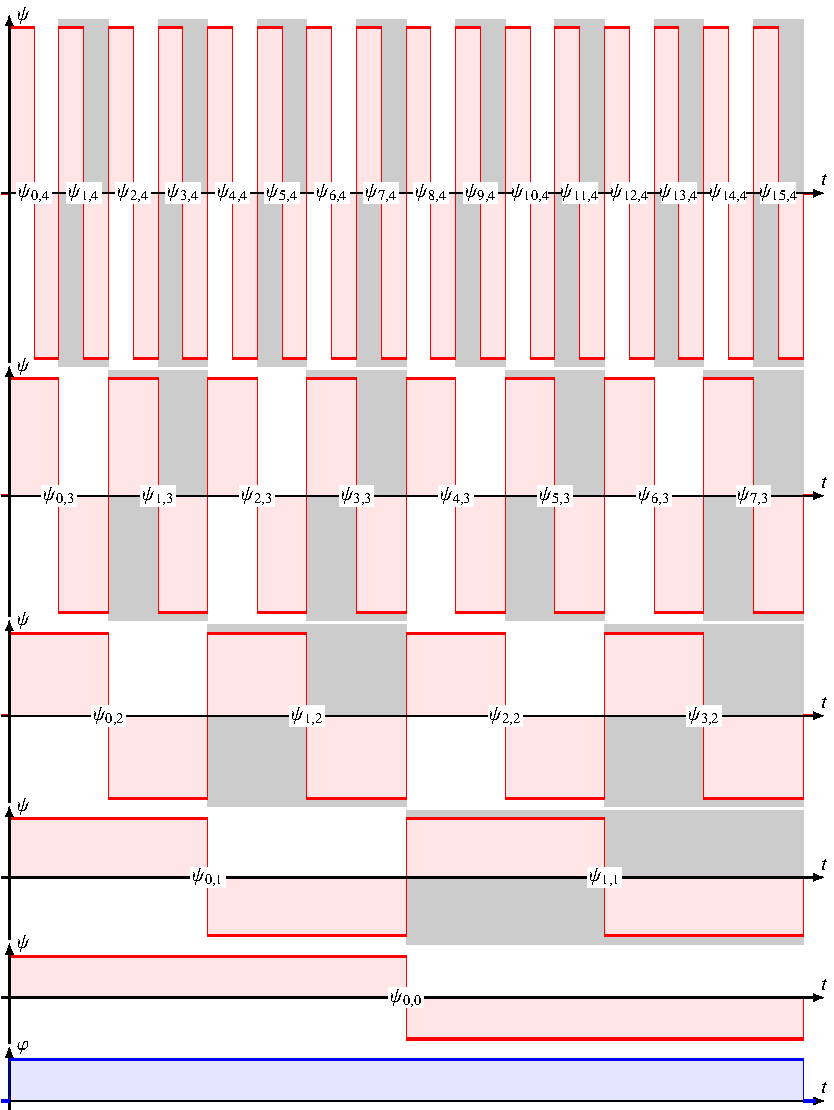
\includegraphics{chapters/3-haar/images/wavelets.pdf}
\caption{Hierarchie der Wavelets $\psi_{jk}$ für das Haar-Wavelet.
In der untersten Zeile ist das Vaterwavelet $\varphi$ dargestellt,
darüber die Wavelets $\psi_{jk}$, wobei die Wavelets mit ungeradem
$j$ jeweils grau hinterlegt sind.
\label{haar:allwavelets:image}}
\end{figure}

Eine Funktion in $V_j$ ist auf ganzzahligen Intervallen der Länge
$2^{-j}$ konstant.
Es muss also nur gezeigt werden, dass das Skalarprodukt von $\psi_{jl}(x)$
mit den charakteristischen Funktionen der Intervalle $[k2^{-j},(k+1)2^{-j})$
verschwindet.
Man rechnet
\[
\langle \chi_{[k2^{-j},(k+1)2^{-j})},\psi_{jl}\rangle
=
\int_{-\infty}^\infty \chi_{[k2^{-j},(k+1)2^{-j})}(x) \psi_{jl}(x)\,dx
=
\int_{k2^{-j}}^{(k+1)2^{-j}} \psi_{jl}(x)\,dx.
\]
Da $\psi_{jl}$ in Intervallen $[k2^{-j},(k+1)2^{-j})$ mit
$k\ne l$ verschwindet, braucht nur der Fall $k=l$ zu untersucht werden.
In diesem Fall gilt
\[
\langle \chi_{[l2^{-j},(l+1)2^{-j})},\psi_{jl}\rangle
=
\int_{l2^{-j}}^{(l+1)2^{-j}} \psi_{jl}(x)\,dx
=
2^{j/2}
\int_{l2^{-j}}^{(l+\frac12)2^{-j}} \,dx
-
2^{j/2}
\int_{(l+\frac12)2^{-j}}^{(l+1)2^{-j}} \,dx
=
2^{j/2}
-
2^{j/2}
=
0,
\]
die Funktionen sind also orthogonal.

\subsection{Erzeugendensystem}
Die Funktionen $\psi_{jl}(x)$ ermöglichen, wirklich alle Funktionen
in $V_{j+1}$ darzustellen.
Um dies einzusehen, muss man nur zeigen, dass sich die Indikatorfunktionen
der Halbintervalle $[l2^{-j},(l+\frac12)2^{-j})$ und
$[(l+\frac12)2^{-j},(l+1)2^{-j})$ linear aus der bereits in $V_j$ vorhandenen
Indikatorfunktion von $[l2^{-j},(l+1)2^{-j})$ und $\psi_{jl}$
kombinieren lässt.
Mit Hilfe der Identität
\[
\chi_{[l2^{-j},(l+1)2^{-j})}
=
\chi_{[l2^{-j},(l+\frac12)2^{-j})}
+
\chi_{[(l+\frac12)2^{-j},(l+1)2^{-j})}
\]
bildet man
\begin{align*}
\chi_{[l2^{-j},(l+1)2^{-j})}
+
2^{-j/2}\psi_{jl}
&=
(
\chi_{[l2^{-j},(l+\frac12)2^{-j})}
+
\chi_{[(l+\frac12)2^{-j},(l+1)2^{-j})}
)
+
(
\chi_{[l2^{-j},(l+\frac12)2^{-j})}
-
\chi_{[(l+\frac12)2^{-j},(l+1)2^{-j})}
)
\\
&=
2
\chi_{[l2^{-j},(l+\frac12)2^{-j})}
\\
\chi_{[l2^{-j},(l+1)2^{-j})}
-
2^{-j/2}\psi_{jl}
&=
(
\chi_{[l2^{-j},(l+\frac12)2^{-j})}
+
\chi_{[(l+\frac12)2^{-j},(l+1)2^{-j})}
)
-
(
\chi_{[l2^{-j},(l+\frac12)2^{-j})}
-
\chi_{[(l+\frac12)2^{-j},(l+1)2^{-j})}
)
\\
&=
2\chi_{[(l+\frac12)2^{-j},(l+1)2^{-j})}.
\end{align*}
Bis auf den Faktor $2$ lassen sich die gesuchten Indikatorfunktionen
aus den $\psi_{jl}$ und gröber aufgelösten Indikatorfunktionen linear
kombinieren.

\subsection{Multiskalenanalyse}
Die Funktionen $\psi_{jl}$ erfassen also genau die Details, die beim
Abtasten mit der feineren Unterteilung mit Korn $2^{-j-1}$ erkennbar
werden.
Aber warum bei $U_0$ beginnen?
Der Mittelwert zweier benachbarter Abtastwerte sagt bereits einiges
über die Werte aus, der Unterschied dieser Werte ist aber das, was
was erst in der Abtastung mit ganzzahligen Abtastpunkten erkennbar wird.
Wir könnten also auch mit $U_{-1}$ beginnen, der Unterteilung
\[
U_{-1} = \{\dots -4,-2,0,2,4,6,8,\cdots\},
\]
und der Menge $V_{-1}$ der stückweise konstanten Funktionen mit
Sprungstellen bei geraden Zahlen.
Doch warum da aufhören: Es gibt eine Zerlegung des Raums der stückweise
konstanten Funktionen mit Sprungstellen in $\mathbb D$ in Form einer
Kette
\begin{equation}
\{0\}
\subset
\dots
\subset
V_{-2}\subset V_{-1} \subset V_{0} \subset V_{2} \subset\dots\subset
V_j \subset V_{j+1}\subset\dots \subset V_{\infty}
\label{haar:kette}
\end{equation}
mit folgenden zum Teil noch nachzuweisenden Eigenschaften:
\begin{enumerate}
% XXX Problem approximation
\item
Jede stückweise konstante Funktion lässt sich beliebig genau
durch Funktionen aus $V_j$ approximieren, also
\[
\bigcup_{j\in\mathbb Z} V_j = V_\infty.
\]
\item
Es gibt eine orthonormierte Familie von Funktionen $\psi_{jl}\in V_{j+1}$,
die auf $V_j$ orthogonal sind, und die genau das erfassen, was in $V_{j+1}$
gegenüber $V_j$ dargestellt werden kann.
Etwas formaler: die $\psi_{jl}$ spannen einen Unterraum
$W_{j} = \langle \psi_{jl}\,|\, l\in\mathbb Z\rangle \subset V_{j+1}$
auf derart, dass
\[
V_{j+1} = V_j \oplus W_j.
\]
\item 
Die Funktionen $\psi_{jl}$ sind Translate einer einzigen Funktion.
Die Funktion $\psi_{jl}$ ist die Verschiebung der Funktion $\psi_{j0}$ 
um $l2^{-j}$.
\item
Die Funktionen $\psi_{j0}$ sind Streckung der Funktion
$\psi_{00}$ um den Faktor $2^{-j}$, die wir auch mit
$\psi(x)=\psi_{00}(x)$ bezeichnen wollen:
\[
\psi_{j0}(x) = \frac1{2^{j/2}}\psi_{00}(2^jx).
\]
$\psi$ heisst das {\em Mutterwavelet}.
\item 
Nur für die Nullfunktion verschwinden alle Abtastungen mit Funktionen
$\psi_{jl}$, oder etwas formeller:
\[
\bigcap_{j\in\mathbb Z} V_j
=
\{0\}.
\]
\end{enumerate}
Man nennt diese Struktur eine Multiskalenanalyse, sie wird im
Kapitel~\ref{chapter:msa} definiert und analysiert.

\subsection{Vaterwavelet}
Die Konstruktion der Funktionen $\psi$ zeigt aber noch eine weitere 
Besonderheit, die später von Nutzen sein wird.
Die $\psi$-Funktionen wurden als Differenzen von charakteristischen
Funktionen von Intervallen mit aufeinanderfolgenden Endpunkten in $U_{j+1}$
aufgebaut.
Alle diese charakteristischen Funktionen sind verschobene und geeignet
gestreckte Versionen der charakteristischen Funktion des Grundintervalls
$[0,1)$.
Setzen wir
\[
\varphi(x) = \chi_{[0,1)} (x),
\]
dann ist
\[
\chi_{[l2^{-j},(l+1)2^{-j})}(x)
=
\varphi(2^jx-l).
\]
% XXX Begründung
Und auch die Funktion $\psi_{00}$, aus der sich alle $\psi_{jl}$ durch
Streckung und Verschiebung gewinnen lassen, lässt sich aus $\varphi$
aufbauen:
\begin{equation}
\psi_{00}(x) = \varphi(2x) - \varphi(2x - 1).
\label{haar:psiphi}
\end{equation}
Die Funktion $\varphi$ heisst auch das {\em Vaterwavelet}.
Das Vaterwavelet $\varphi$ erfüllt eine ähnliche Relation
wie \eqref{haar:psiphi}.
Bei der Konstruktion haben wir diese Relation sogar in entscheidender
Weise gebraucht, indem wir das Intervall in zwei Halbintervalle aufgeteilt
haben.
Diese Aufteilung bedeutet
\[
\varphi(x) = \varphi(2x) + \varphi(2x-1),
\]
bis auf das Vorzeichen des zweiten Summanden dasselbe wie 
\eqref{haar:psiphi}.

Das Vaterwavelet und seine ganzzahlig verschobenen Kopien bilden
eine Basis des Vektorraumes $V_0$.
Schreiben wir $\varphi_k(x)=\varphi(x-k)$, dann ist
\[
V_0 = \langle \varphi_k\,|\, k\in\mathbb Z\rangle.
\]
Die feiner aufgelösten Funktionen $V_j$ haben die gestauchten Funktionen
$\tilde{D}_{2^j}\varphi_K$ mit
$(\tilde{D}_{2^j}\varphi_k)(x)=\varphi_k(2^jx)$ als Basis.
Diese sind zwar orthogonal, aber erst $2^{j/2}\varphi_k(2^jx)$ sind
orthonormiert.
Die Funktionen $\varphi$ und $\psi$ liefern daher die Zerlegung
des Raumes
\[
V_1
=
V_0 \oplus W_1
=
\langle \varphi_k\,|\,k\in\mathbb Z\rangle
\oplus
\langle \psi_k\,|\,k\in\mathbb Z\rangle
\]
in zwei orthogonale Teilräume.

\subsection{Verallgemeinerung}
Aus diesem Beispiel können wir einen Plan für die Konstruktion allgemeinerer
Waveletbasen ableiten.
Wir hätten gerne eine Aufteilung des interessierenden Funktionenraumes
in Form einer Kette \eqref{haar:kette} derart, dass die ``Zwischenräume''
$W_j$ eine Orthonormalbasis haben, die aus verschobenen und gestreckten
Kopien
$\psi()$
einer einzigen Funktion $\psi$, dem Mutterwavelet, besteht.
Das Mutterwavelet ist eine Linearkombination von verschobenen
und skalierten Kopien des Vaterwavelets $\varphi(x)$, welches seinerseits
eine Linearkombination von verschobenen und skalierten Kopien seiner
selbst ist.
Die Koeffizienten der Linearkombinationen für $\psi$ und $\varphi$ sind
bis auf die Vorzeichen identisch.




